\section{Desarrollo}
\label{sec:desarrollo}

\subsection{Estructura.}

\subsubsection{Proyecto.}

La estructura de la aplicación procura seguir cuidadosamente el patrón MVVM y las mejores prácticas de Android, organizando el código en módulos que facilitan el mantenimiento, la escalabilidad y la comprensión del sistema. La organización del proyecto se define de la siguiente manera:

\begin{itemize}
    \item \textbf{config:} Contiene las configuraciones de la base de datos Room, así como futuros archivos de configuración que pueda necesitar el proyecto.
    
    \item \textbf{di:} Implementa la inyección de dependencias utilizando Dagger-Hilt, siguiendo las recomendaciones de Google para la gestión de dependencias en Android. Hilt facilita la creación y provisión automática de instancias de UseCases y ViewModels.
    
    \item \textbf{events:} Define los eventos de la aplicación que permite la coordinación entre la UI, los ViewModels y la gestión de estados.
    
    \item \textbf{model:} Contiene las entidades de la base de datos que representan la estructura de información del launcher. Incluye modelos para tareas, hábitos, aplicaciones, límites y categorías, cada uno definiendo la estructura de datos específica para su dominio correspondiente mediante anotaciones de Room. Además, incluye clases de estado auxiliares, constantes usadas a lo largo del proyecto y la lógica de negocio encapsulada en UseCases, que representan las operaciones que pueden realizarse sobre los datos, como añadir, eliminar o actualizar tareas y hábitos.
    
    \item \textbf{navigation:} Gestiona la navegación entre pantallas utilizando \textit{Navigation Compose} de Jetpack, proporcionando una navegación fluida y consistente a través de toda la aplicación. Define las rutas de navegación y maneja las transiciones entre diferentes vistas del launcher.
    
    \item \textbf{services:} Implementa servicios especializados para límite de tiempo de aplicaciones, gestión de notificaciones del sistema y actualización de estado de tareas y hábitos al inicio de cada día.
    
    \item \textbf{utils:} Proporciona utilidades y funciones auxiliares reutilizables a lo largo del proyecto.
    
    \item \textbf{view:} Representa la capa de vista implementada completamente en Jetpack Compose. Esta carpeta se subdivide en módulos específicos que incluyen componentes reutilizables, pantallas principales y vistas especializadas para la gestión de elementos. Cada vista observa los cambios en su ViewModel correspondiente y se recompone automáticamente según el estado de la aplicación.
    
    \item \textbf{viewmodel:} Constituye el núcleo del patrón MVVM, implementando los ViewModels específicos para cada funcionalidad principal. Cada ViewModel gestiona el estado y la lógica de presentación de su respectiva vista mediante StateFlow y corrutinas de Kotlin.
\end{itemize}

\subsubsection{Base de datos.}

El modelo de datos del launcher se compone de seis entidades principales, cada una diseñada para encapsular un aspecto específico de la funcionalidad del launcher:

\begin{itemize}
  \item \textbf{ApplicationsModel:} Entidad para gestionar las aplicaciones instaladas en el dispositivo. Esta almacena información esencial sobre cada aplicación que el usuario puede controlar a través del launcher.
  \item \textbf{TasksModel:} Representa las tareas que el usuario puede crear y gestionar dentro del launcher como parte de su sistema de productividad personal.
  \item \textbf{HabitsModel:} Contiene la información relacionada con los hábitos que el usuario desea formar o mantener como parte de su rutina diaria. Esta entidad sigue una estructura similar a las tareas pero está optimizada para el seguimiento a largo plazo.
  \item \textbf{HabitsLogsModel:} Implementa el sistema de seguimiento temporal para los hábitos, permitiendo el registro histórico del cumplimiento de cada hábito a lo largo del tiempo. Esta implementación permite análisis de tendencias y proporciona al usuario retroalimentación sobre su progreso en la formación de hábitos. Aunque fue implementada, no se utilizó en la versión final del launcher, sino que hace parte de trabajos futuros \textbf{REFERENCIA A TRABAJOS FUTUROS}.
  \item \textbf{CategoriesModel:} Este modelo permite al usuario asignar una etiqueta a tareas y hábitos relacionados.
  \item \textbf{LimitsModel:} Gestiona las restricciones de tiempo que el usuario puede establecer para aplicaciones específicas como parte del sistema de control de uso del dispositivo.
\end{itemize}


La relación entre estas entidades y sus atributos se ilustra en la Figura \ref{fig:diagrama_uml}.

\begin{figure}[ht]
  \caption{Diagrama de la base de datos del launcher.}
  \label{fig:diagrama_uml}
  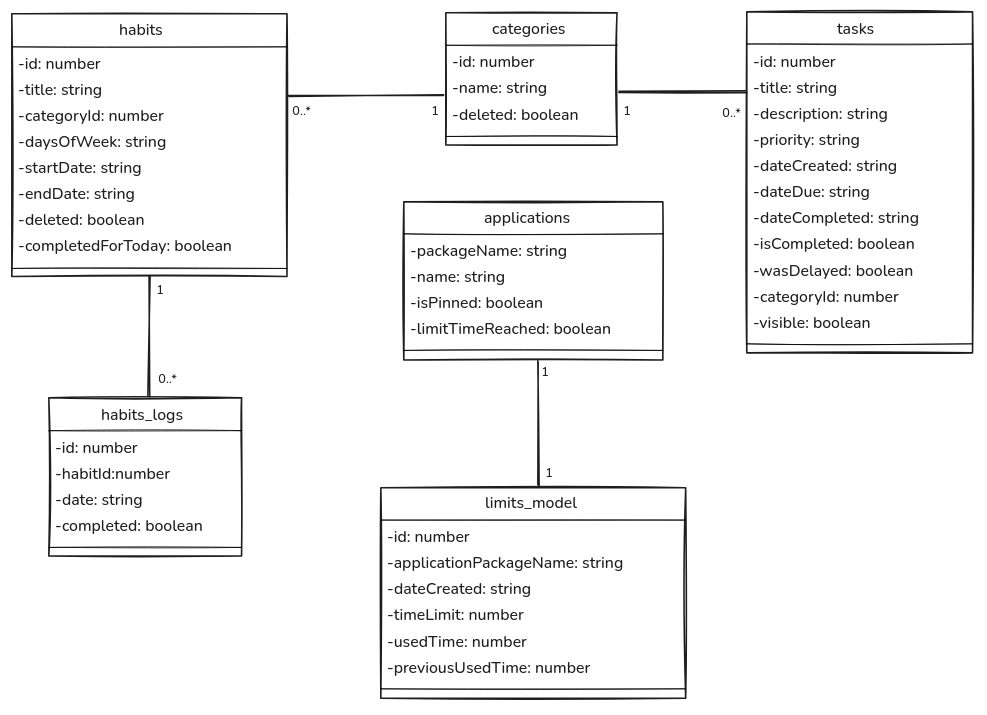
\includegraphics[width=\textwidth]{Figuras/diagrama_uml.png}
  \centering
\end{figure}